\documentclass[11pt,a4paper]{article}

\usepackage[T1]{fontenc}
\usepackage[utf8]{inputenc}
\usepackage[margin=2.3cm]{geometry}
\usepackage{lmodern}
\usepackage{graphicx}
\usepackage{booktabs}
\usepackage{longtable}
\usepackage{array}
\usepackage{xcolor}
\usepackage{listings}
\usepackage{float}
\usepackage{enumitem}
\usepackage{fancyhdr}
\usepackage[colorlinks=true,linkcolor=blue!50!black,urlcolor=blue!50!black]{hyperref}

\definecolor{codebg}{RGB}{245,246,248}
\lstset{
  basicstyle=\ttfamily\footnotesize,
  backgroundcolor=\color{codebg},
  frame=single,
  rulecolor=\color{black!20},
  breaklines=true,
  breakatwhitespace=false,
  columns=fullflexible,
  keepspaces=true,
  showstringspaces=false,
  aboveskip=8pt,
  belowskip=8pt
}

\setlength{\parindent}{0pt}
\setlength{\parskip}{6pt}
\setlist{itemsep=2pt,topsep=4pt}
\renewcommand{\arraystretch}{1.25}

\pagestyle{fancy}
\fancyhf{}
\fancyhead[L]{SysOps Practical Examination}
\fancyhead[R]{Nimesha Yasith}
\fancyfoot[C]{\thepage}

\newcommand{\code}[1]{\texttt{#1}}

\title{\textbf{SysOps Engineer Practical Examination}\\[4pt]
\large Three PHP Websites on AWS with Nginx and Amazon RDS}
\author{Nimesha Yasith}
\date{16 November 2026}

\begin{document}
\maketitle

\begin{abstract}
This report documents the design, build and verification of a hosting platform on AWS
(region \code{ap-southeast-1}). A dedicated VPC contains one Ubuntu 24.04 web server
running Nginx and PHP 8.3-FPM that serves three PHP websites. Each website uses its own
database on a private Amazon RDS MySQL instance. The network, security groups, EC2 instance
and database are created with Terraform. The report lists what was built, the evidence that
it works, and the problems met along the way.
\end{abstract}

\tableofcontents
\newpage

%------------------------------------------------------------
\section{Overview}
%------------------------------------------------------------
A client needs three small PHP websites hosted cheaply on one server, each with its own
MySQL database. Only the web server is reachable from the internet. The database sits in
private subnets and accepts connections from the web server alone.

\begin{table}[H]
\centering
\begin{tabular}{@{}ll@{}}
\toprule
\textbf{Item} & \textbf{Value}\\
\midrule
Region & \code{ap-southeast-1} (Singapore)\\
Web server & \code{sysops-nimesha-web01}, Elastic IP \code{47.130.163.143}\\
Database & \code{sysops-nimesha-db}, MySQL 8.0, \code{db.t3.micro}, single-AZ, private\\
Tags on all resources & \code{Project = SysOpsTest}, \code{Owner = Nimesha Yasith}\\
Resource name prefix & \code{sysops-nimesha-}\\
\bottomrule
\end{tabular}
\caption{Project summary.}
\end{table}

%------------------------------------------------------------
\section{Architecture}
%------------------------------------------------------------
\begin{lstlisting}
Visitors --HTTP/HTTPS--> Internet Gateway
                              |
 VPC sysops-nimesha-vpc 10.10.0.0/16
  AZ ap-southeast-1a                    AZ ap-southeast-1b
  Public subnet A 10.10.1.0/24          Public subnet B 10.10.2.0/24 (spare)
   EC2 t3.micro, Ubuntu 24.04
   Nginx + PHP 8.3-FPM
   website1 | website2 | website3
   web-sg: 80,443 any; 22 my IP
        | MySQL 3306 (db-sg: from web-sg only)
  Private subnet A 10.10.11.0/24        Private subnet B 10.10.12.0/24
   RDS MySQL 8.0 db.t3.micro             (second AZ for the DB subnet group)
   site1_db | site2_db | site3_db
\end{lstlisting}

%------------------------------------------------------------
\section{Implementation}
%------------------------------------------------------------
\subsection{Network (Task 1)}
\begin{table}[H]
\centering
\begin{tabular}{@{}p{3.6cm}p{11cm}@{}}
\toprule
\textbf{Resource} & \textbf{Configuration}\\
\midrule
VPC & \code{sysops-nimesha-vpc}, \code{10.10.0.0/16}, DNS support and hostnames enabled; the default VPC is not used\\
Public subnets & \code{10.10.1.0/24} (1a) and \code{10.10.2.0/24} (1b), auto-assign public IPv4 on\\
Private subnets & \code{10.10.11.0/24} (1a) and \code{10.10.12.0/24} (1b)\\
Internet gateway & Attached to the VPC\\
Public route table & \code{0.0.0.0/0} to the gateway, associated with both public subnets\\
Private route table & Local route only, associated with both private subnets\\
NAT gateway & None\\
\bottomrule
\end{tabular}
\caption{Network resources.}
\end{table}

\subsection{Security groups (Task 2)}
\begin{table}[H]
\centering
\begin{tabular}{@{}p{4.6cm}p{10cm}@{}}
\toprule
\textbf{Group} & \textbf{Inbound rules}\\
\midrule
\code{sysops-nimesha-web-sg} & TCP 80 and 443 from \code{0.0.0.0/0}; TCP 22 from the administrator's single address (\code{/32})\\
\code{sysops-nimesha-db-sg} & TCP 3306 from \code{web-sg} only, referenced by security group rather than by CIDR range\\
\bottomrule
\end{tabular}
\caption{Security groups.}
\end{table}
The web group also has an allow-all outbound rule. Terraform removes AWS's default
outbound rule, and the server needs outbound access for package updates and for its
connection to the database.

\subsection{Web server (Tasks 3 and 4)}
Ubuntu Server 24.04 LTS on a \code{t3.micro} in public subnet A, with a new key pair, a
20\,GiB encrypted \code{gp3} root volume, IMDSv2 required and an Elastic IP. The hostname is
\code{sysops-web01} and the timezone is \code{Asia/Colombo}.

Installed packages: \code{nginx}, \code{php8.3-fpm}, \code{php8.3-mysql}, \code{php8.3-cli},
\code{php8.3-mbstring}, \code{php8.3-xml} and \code{mysql-client}. Nginx passes PHP requests
to PHP-FPM through the Unix socket \code{/run/php/php8.3-fpm.sock}, and both services start
at boot. Hardening: \code{server\_tokens off;} in Nginx and \code{expose\_php = Off} in PHP.

\subsection{Database (Tasks 5 and 6)}
\begin{itemize}
  \item MySQL 8.0, \code{db.t3.micro}, single-AZ, 20\,GiB encrypted \code{gp3}.
  \item Public access disabled; security group \code{db-sg} only.
  \item Automated backups on with 1-day retention; deletion protection off so the
        evaluator can remove it.
  \item A DB subnet group spans the two private subnets.
  \item A SQL script creates the databases \code{site1\_db}, \code{site2\_db} and
        \code{site3\_db} and one user per database, each limited to its own database.
\end{itemize}

\subsection{Virtual hosts (Task 7)}
\begin{table}[H]
\centering
\begin{tabular}{@{}lll@{}}
\toprule
\textbf{Domain} & \textbf{Document root} & \textbf{Database}\\
\midrule
\code{website1.saberion.cloud} & \code{/var/www/website1.saberion.cloud/public} & \code{site1\_db}\\
\code{website2.saberion.cloud} & \code{/var/www/website2.saberion.cloud/public} & \code{site2\_db}\\
\code{website3.saberion.cloud} & \code{/var/www/website3.saberion.cloud/public} & \code{site3\_db}\\
\bottomrule
\end{tabular}
\caption{Virtual hosts.}
\end{table}
Each domain has its own server block in \code{sites-available/}, enabled with a symlink, and
its own access and error log. The default site is removed. A \code{default\_server} block
returns \code{444}, so the bare IP address and unknown host names show none of the sites.
Only \code{public/} is served. The file \code{config.php} sits one level above it, owned by
\code{root:www-data} with mode \code{640}, so PHP-FPM can read it but other users cannot.

\subsection{Websites (Task 8)}
\begin{table}[H]
\centering
\begin{tabular}{@{}p{4.4cm}p{3.3cm}p{6.8cm}@{}}
\toprule
\textbf{Site} & \textbf{Type} & \textbf{Content read from its own database}\\
\midrule
Website 1: Northwind Digital & Company website & News items\\
Website 2: Cartly Shop & Online shop & Products, shopping cart and checkout (tables \code{cart\_items}, \code{orders}, \code{order\_items})\\
Website 3: BrightPath Learning & Learning system & Courses\\
\bottomrule
\end{tabular}
\caption{The three websites.}
\end{table}
Each site has a dynamic \code{index.php} as its default page and a static \code{about.html}
served directly by Nginx. A \emph{System status} panel in the footer shows \textbf{Connected},
the site name, the message stored in that site's own database, and a visit counter that
rises on every refresh. The shop's forms use CSRF tokens and prepared statements, and prices
are always read from the database, never from the browser. Database passwords are stored
only in each site's \code{config.php} on the server.

%------------------------------------------------------------
\section{Verification and evidence}
%------------------------------------------------------------
Evidence was collected on 16 November 2026 with the AWS CLI, \code{curl} and Chrome against
the Elastic IP.

\subsection{Infrastructure}
\begin{table}[H]
\centering
\begin{tabular}{@{}p{5.4cm}p{9.2cm}@{}}
\toprule
\textbf{Check} & \textbf{Result}\\
\midrule
Instance type, zone, subnet & \code{t3.micro}, \code{ap-southeast-1a}, public subnet A\\
Instance metadata & IMDSv2 required\\
Root volume & 20\,GiB, \code{gp3}, encrypted\\
Elastic IP & \code{47.130.163.143}, attached to the instance\\
Security group on instance & \code{sysops-nimesha-web-sg}\\
Subnets & All four CIDRs correct; public subnets auto-assign IPs, private do not\\
NAT gateways & None\\
Private route table & Local route only; two subnet associations\\
Public route table & \code{0.0.0.0/0} to the gateway; two subnet associations\\
\code{db-sg} inbound & 3306 from \code{web-sg} only\\
RDS & MySQL 8.0.46, \code{db.t3.micro}, single-AZ, 20\,GiB \code{gp3}, encrypted, not public, 1-day backups, deletion protection off, status \emph{available}\\
Tags & \code{Project = SysOpsTest}, \code{Owner = Nimesha Yasith}\\
\bottomrule
\end{tabular}
\caption{Infrastructure checks (AWS CLI).}
\end{table}

\subsection{Web behaviour}
\begin{table}[H]
\centering
\begin{tabular}{@{}p{4.6cm}p{3.8cm}p{6.2cm}@{}}
\toprule
\textbf{Check} & \textbf{Expected} & \textbf{Result}\\
\midrule
Request to the bare IP & No site shown & Connection closed, no reply (\code{444})\\
Unknown host name & No site shown & Connection closed, no reply (\code{444})\\
\code{/config.php} on each site & Not downloadable & HTTP 404 on all three\\
Response headers & No version shown & \code{Server: nginx}, no \code{X-Powered-By}\\
Each home page & Connected, own site and message & Passed on all three sites\\
Refresh the page & Visit count rises & Website 3 went from 8 to 9\\
\bottomrule
\end{tabular}
\caption{Web checks (\code{curl}).}
\end{table}

\subsection{Screenshots}
\begin{figure}[H]
\centering
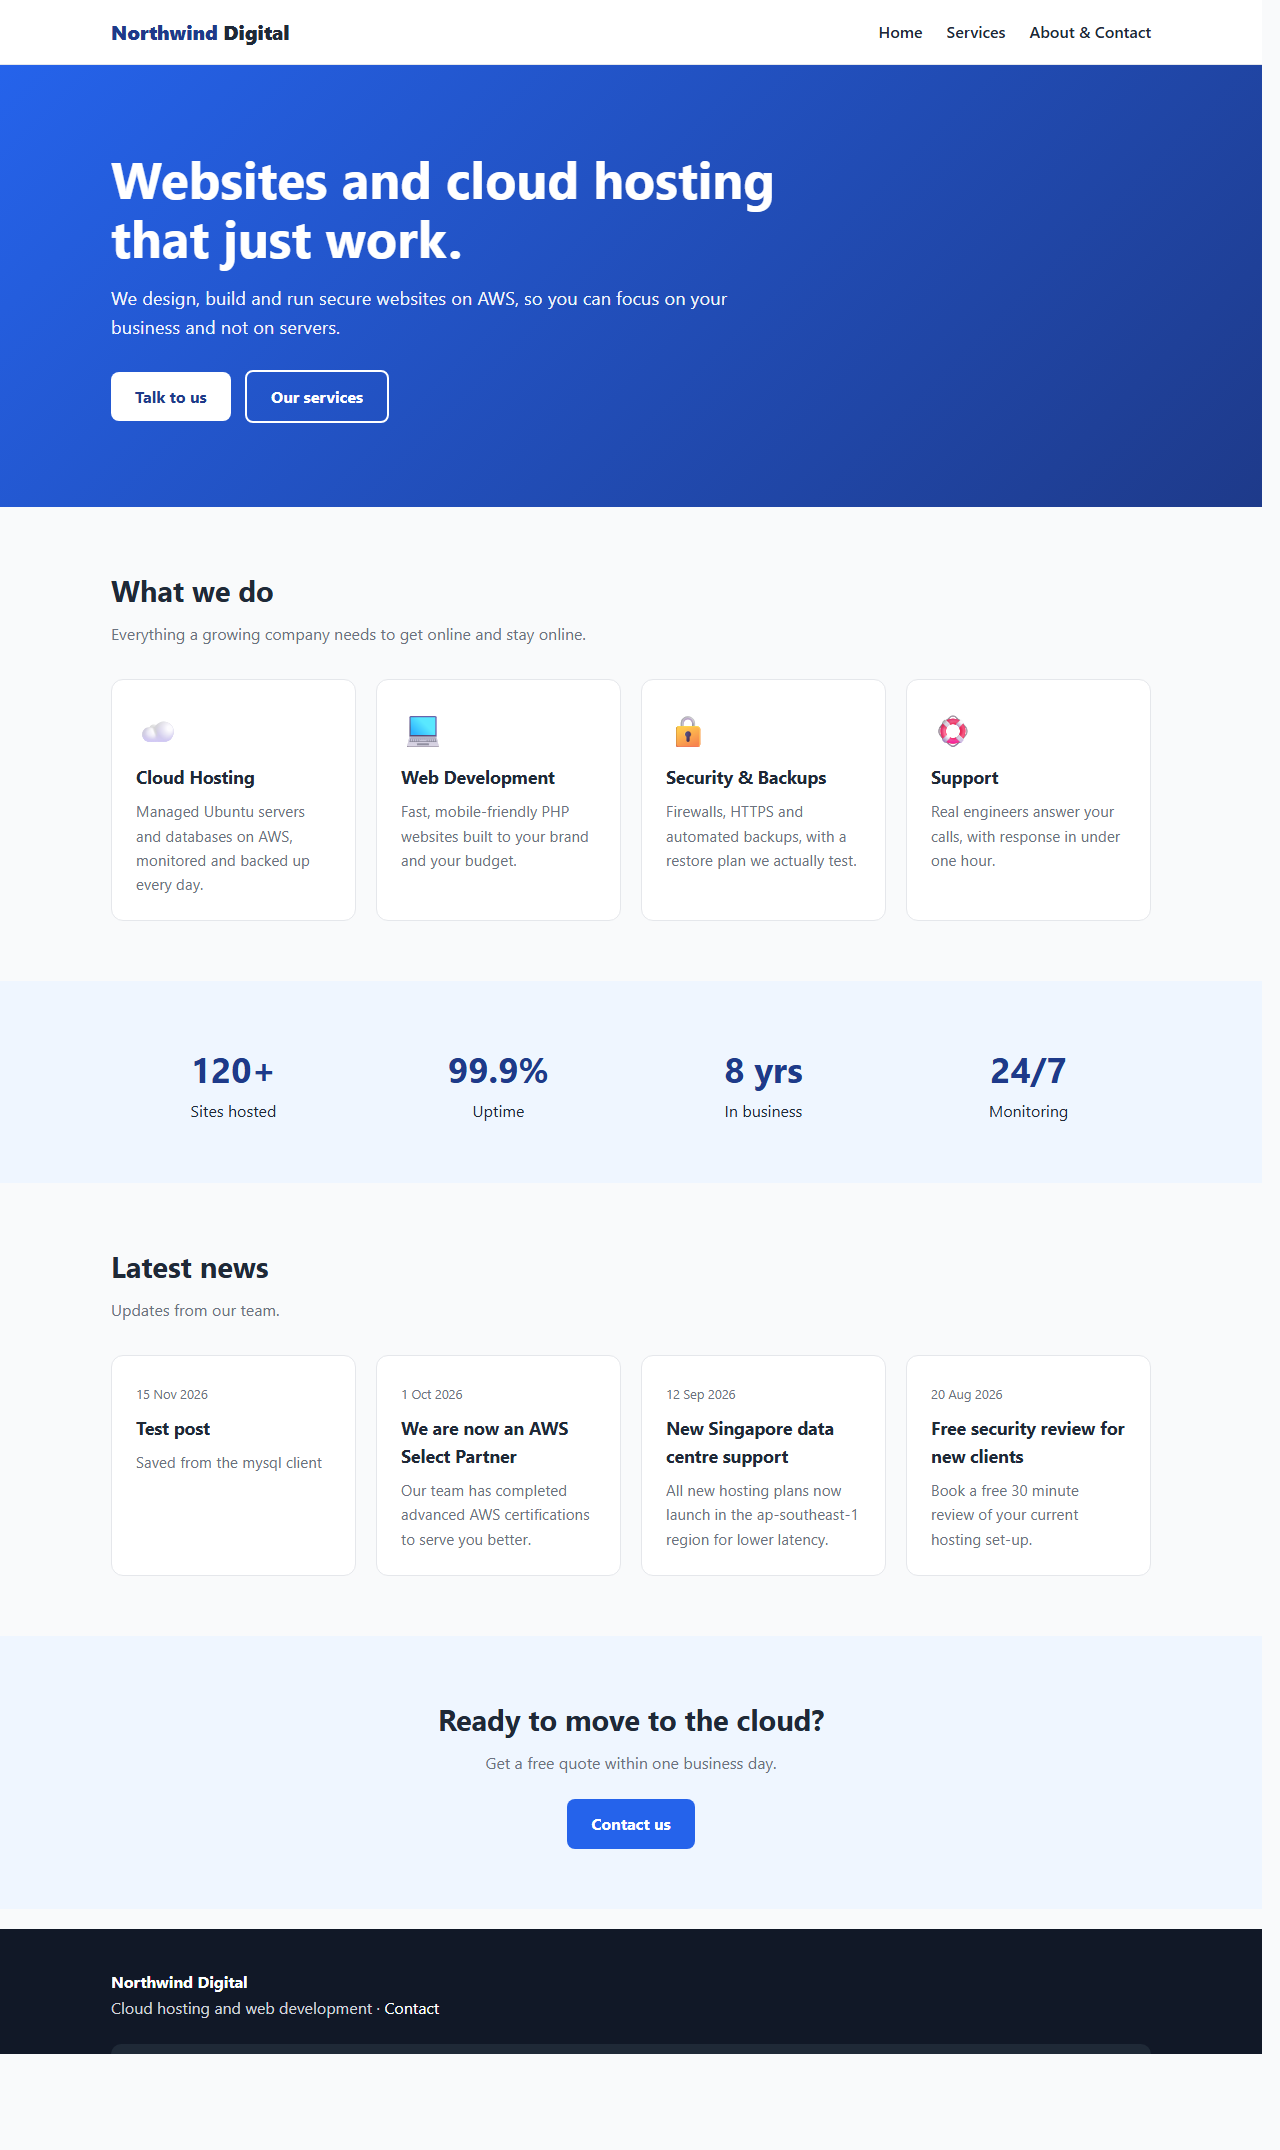
\includegraphics[height=0.78\textheight,keepaspectratio]{images/website1-home.png}
\caption{Website 1, Northwind Digital, with the status panel in the footer.}
\end{figure}

\begin{figure}[H]
\centering
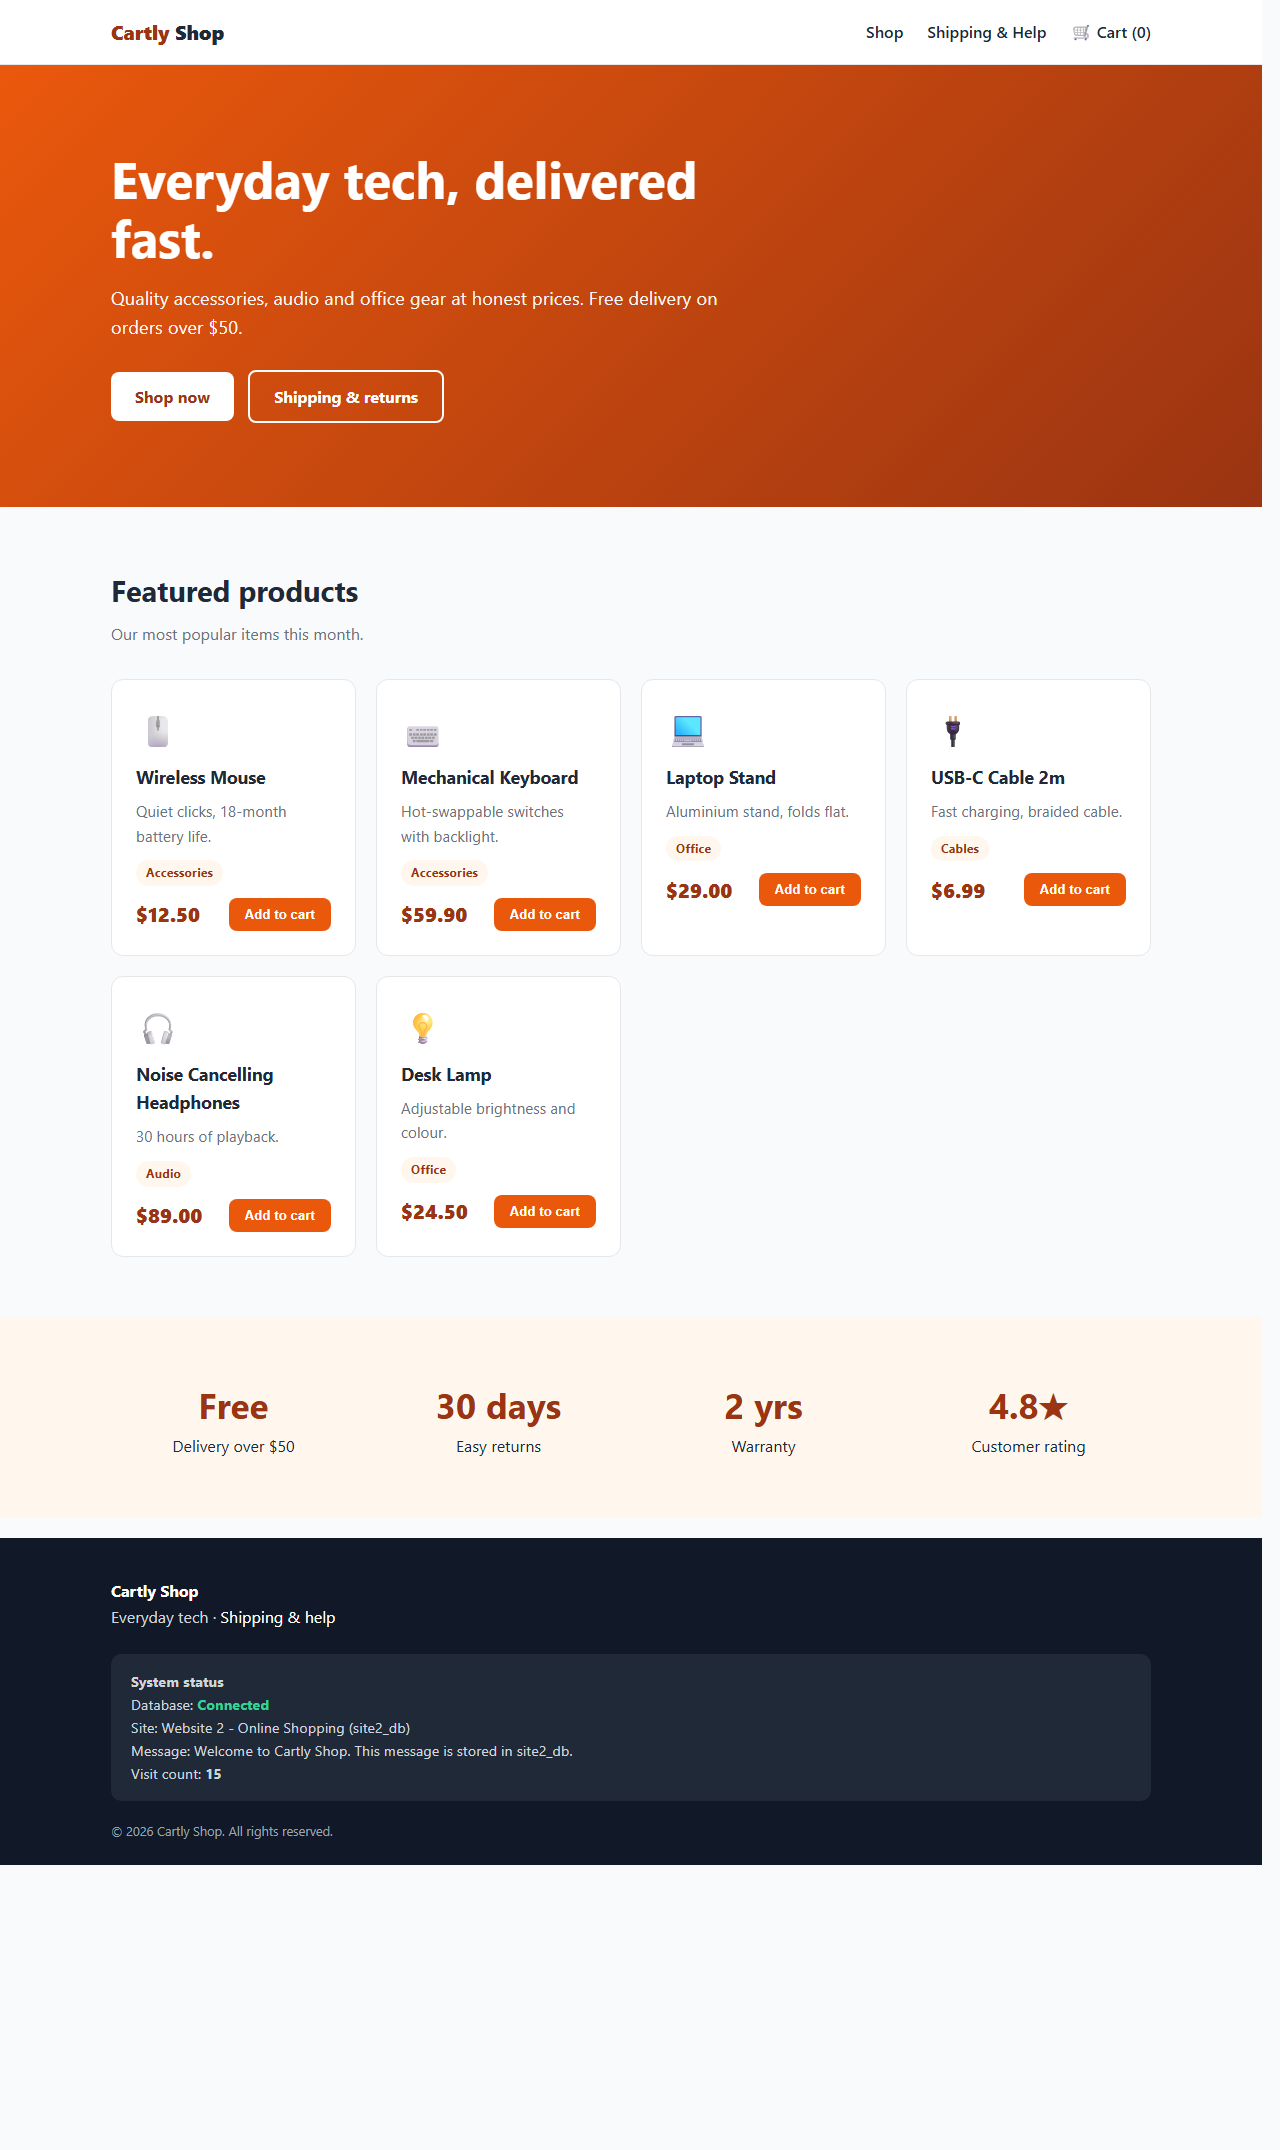
\includegraphics[height=0.78\textheight,keepaspectratio]{images/website2-home.png}
\caption{Website 2, Cartly Shop. The footer shows \emph{Connected}, \code{site2\_db} and the visit count.}
\end{figure}

\begin{figure}[H]
\centering
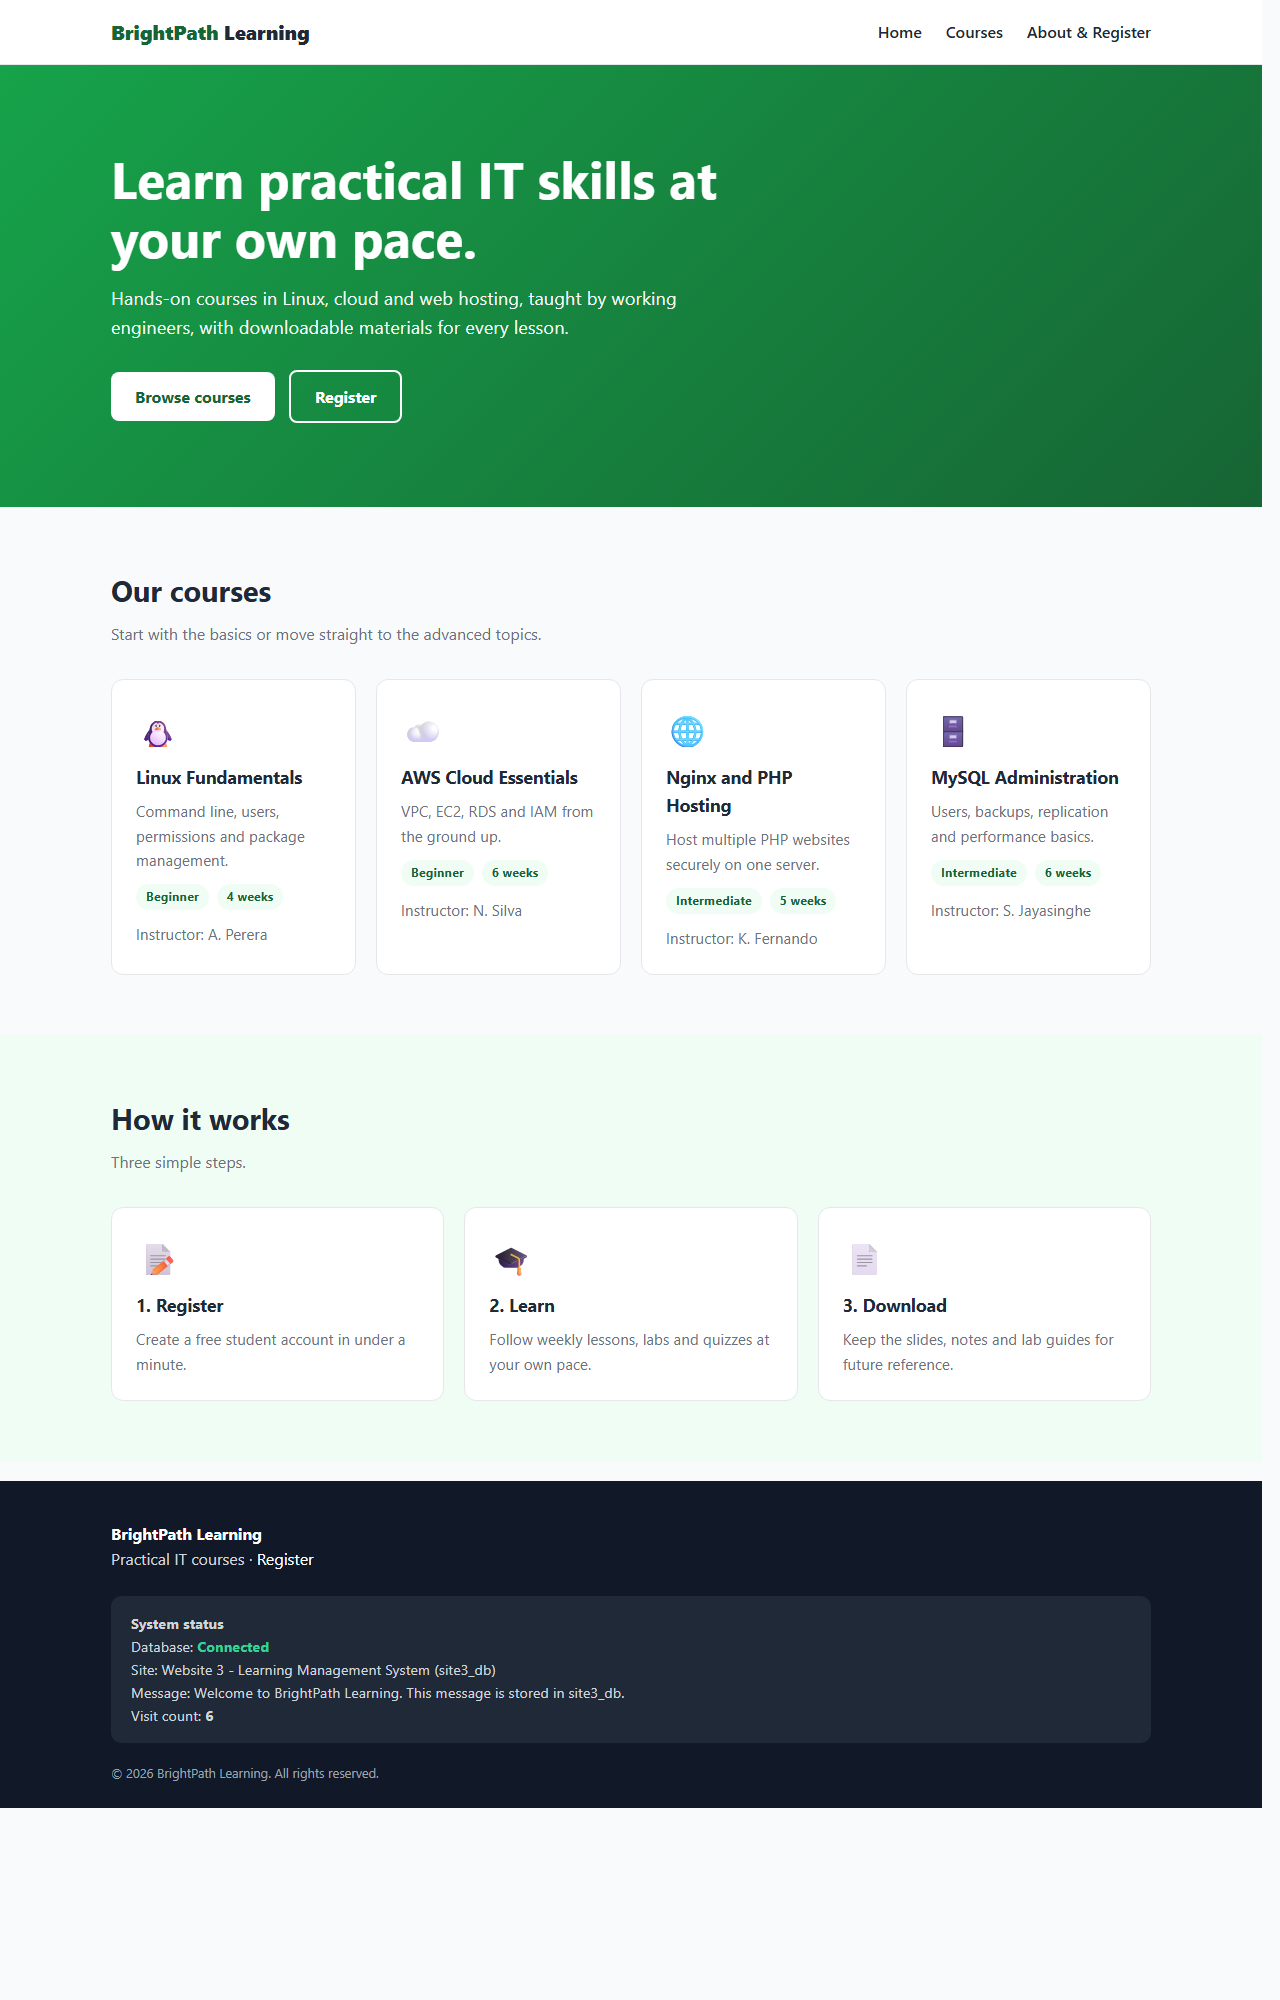
\includegraphics[height=0.78\textheight,keepaspectratio]{images/website3-home.png}
\caption{Website 3, BrightPath Learning.}
\end{figure}

\begin{figure}[H]
\centering
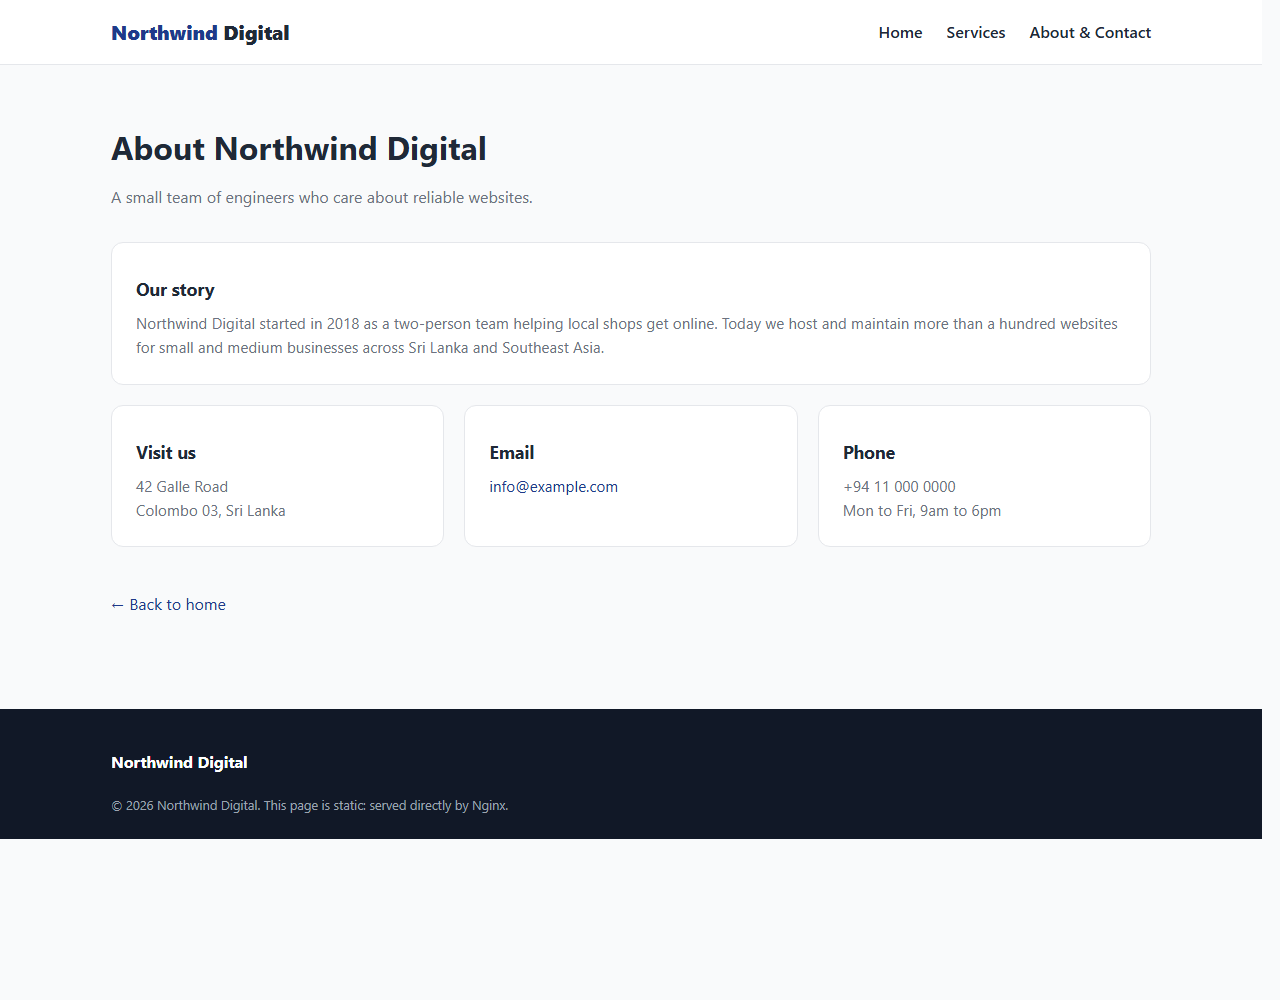
\includegraphics[width=0.85\linewidth]{images/website1-about.png}
\caption{A static page, served directly by Nginx without PHP or the database.}
\end{figure}

\begin{figure}[H]
\centering
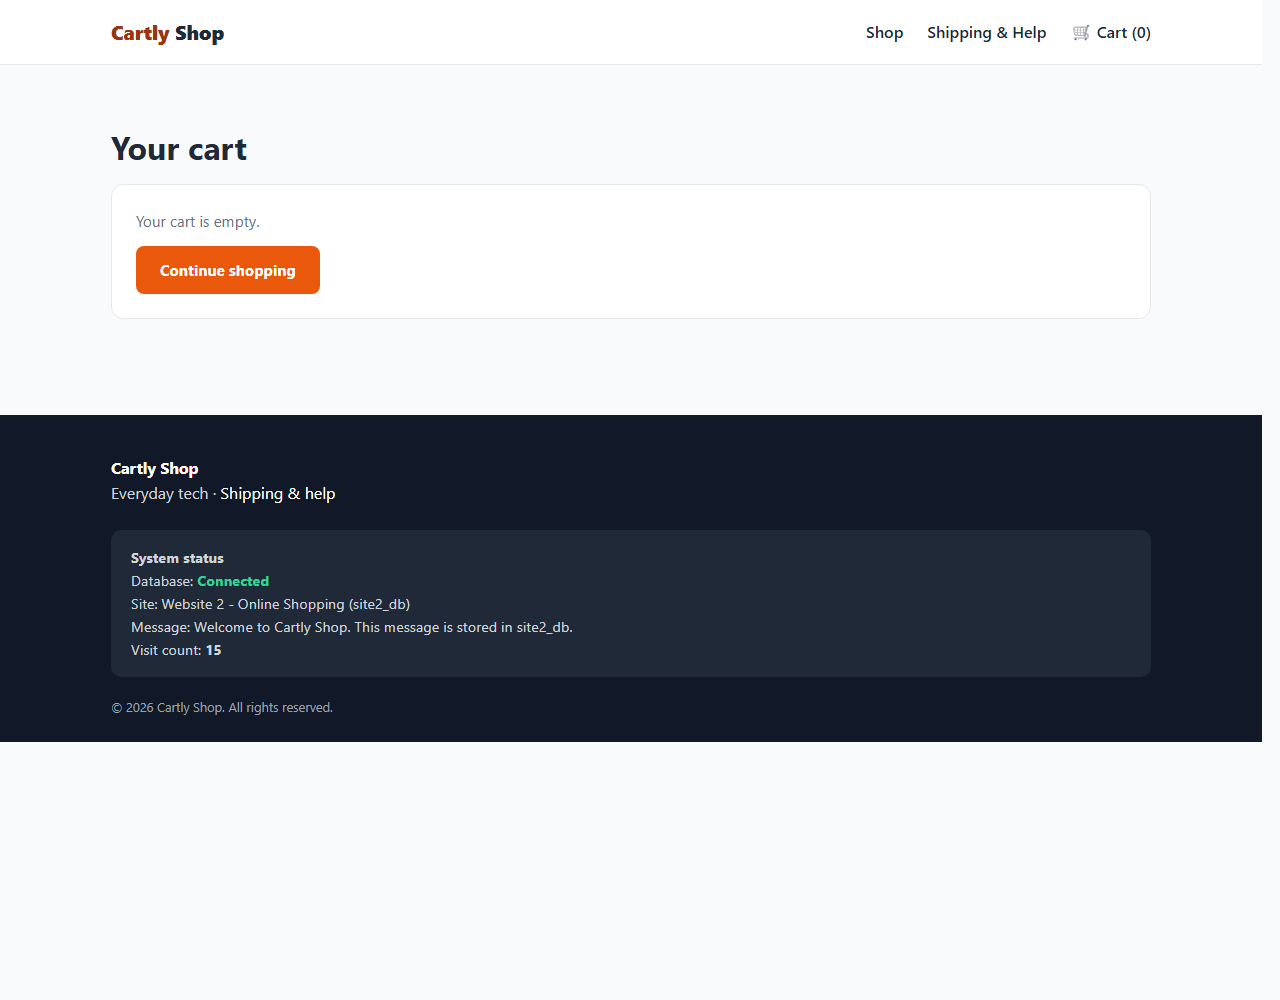
\includegraphics[width=0.85\linewidth]{images/website2-cart.png}
\caption{The shopping cart page of Website 2.}
\end{figure}

\subsection{Server-side evidence to add}
Run these on the server and paste the output into the work log.
\begin{lstlisting}
nginx -v; php -v
systemctl is-enabled nginx php8.3-fpm
sudo nginx -t
hostnamectl | grep -i "static hostname"; timedatectl | grep "Time zone"
ls -l /var/www/website*.saberion.cloud/config.php
mysql --no-defaults -h <rds-endpoint> -u site1_user -p -e "USE site2_db"
\end{lstlisting}
The last command must fail with \emph{Access denied}, which proves each user can reach only
its own database.

%------------------------------------------------------------
\section{Work log: problems and fixes}
%------------------------------------------------------------
\begin{longtable}{@{}p{4.3cm}p{4.6cm}p{5.4cm}@{}}
\toprule
\textbf{Problem} & \textbf{Cause} & \textbf{Fix}\\
\midrule
\endhead
Terraform differed from the exam requirements & Apache instead of Nginx; 0-day backups; names without the \code{sysops-<firstname>-} prefix; no explicit private route table & Added a \code{name\_prefix} variable, set backups to 1 day, pinned MySQL 8.0, added a private route table\\
Old \code{web-sg} could not be deleted (\code{DependencyViolation}) & Terraform removed the group before moving the instance to the new one & Added \code{create\_before\_destroy} to both security groups\\
\code{apt install mysql-client} timed out & Terraform removes the default outbound rule, so the web group had no egress & Added an allow-all outbound rule to the web group\\
\code{terraform plan} failed with a state lock & An earlier background plan still held the state file & Waited for it to finish and ran again\\
Error \emph{no such host} for the RDS API & Local DNS problem on the laptop & Retried once the connection recovered\\
\code{mysql} command not found & Client not installed on the server & \code{sudo apt install mysql-client}\\
\code{export VAR = value} failed & Spaces around the equals sign in Bash & \code{export VAR='value'}\\
Password with \# in \code{.my.cnf} & \# starts a comment in MySQL option files & Wrapped the password in double quotes\\
Password with \code{@} rejected by RDS & RDS disallows \code{@}, \code{/}, \code{"} and spaces & Chose a compliant password\\
\bottomrule
\end{longtable}

%------------------------------------------------------------
\section{Security notes}
%------------------------------------------------------------
\begin{itemize}
  \item Only ports 80, 443 and 22 (from the administrator's IP) are open to the internet;
        the database is private.
  \item Database passwords are stored only in \code{config.php} on the server
        (\code{root:www-data}, mode \code{640}), never in Git or the web root.
  \item The RDS master password also exists in the Terraform state file, which is excluded
        from Git and must be kept private.
  \item The shop uses CSRF tokens, prepared statements, server-side price lookup and
        escaped output.
  \item The master password should be rotated before hand-in if it was ever shared outside
        the terminal.
\end{itemize}

%------------------------------------------------------------
\section{Hand-in notes}
%------------------------------------------------------------
\begin{itemize}
  \item \textbf{DNS:} there is no access to the \code{saberion.cloud} hosted zone. Create A
        records for \code{website1}, \code{website2} and \code{website3} pointing to
        \code{47.130.163.143}, or test with
        \code{curl -H "Host: website1.saberion.cloud" http://47.130.163.143/}.
  \item \textbf{Cleanup:} nothing was deleted. \code{terraform destroy} removes the setup;
        the database has no final snapshot.
  \item \textbf{Optional tasks not done:} HTTPS with certbot (needs real DNS), SSM Session
        Manager, and a CloudWatch agent with a CPU alarm.
\end{itemize}

\end{document}
